\documentclass{article}
\usepackage[polish]{babel}
\usepackage[T1]{fontenc}
\usepackage{float}
\usepackage{subcaption}
\usepackage{caption}
\usepackage[a4paper,top=2cm,bottom=2cm,left=3cm,right=3cm,marginparwidth=1.75cm]{geometry}
\usepackage{amsmath}
\usepackage{graphicx}
\usepackage{hyperref}

\title{Uruchomienie algorytmów wyznaczania trasy dla sieci drogowej}
\author{Adrian Fabisiewicz (328935), Julia Gomulska (328936)}

\begin{document}
\maketitle
\renewcommand{\labelenumii}{\arabic{enumi}.\arabic{enumii}}
\renewcommand{\labelenumiii}{\arabic{enumi}.\arabic{enumii}.\arabic{enumiii}}
\renewcommand{\labelenumiv}{\arabic{enumi}.\arabic{enumii}.\arabic{enumiii}.\arabic{enumiv}}

\section{Opis ćwiczenia}

Celem ćwiczenia było uruchomienie algorytmów wyznaczania trasy dla sieci drogowej. W ramach ćwiczenia zaimplementowano algorytm A*. Stworzony program odczytuje sieć drogową z wybranego źródła oraz uruchamia wyznaczanie trasy pomiędzy dwoma punktami, uwzględniając kierunkowość dróg. Następnie zwraca trasę najkrótszą oraz najszybszą. Program zintegrowano z oprogramowaniem GIS - ArcGIS Pro, dzięki czemu użytkownik ma możliwość ręcznego wybrania punktów początkowego i końcowego na mapie. Zaimplementowano również rozszerzenie, pozwalające na wyznaczenie zasięgu obszaru, do którego można dojechać z danego punktu w określonym czasie.

\section{Środowisko pracy oraz wykorzystane dane}
Ćwiczenie zostało wykonane w języku Python z wykorzystaniem biblioteki ArcPy. Do kontroli wersji korzystano z systemu Git. Danymi wejściowymi były dane BDOT dla Torunia i powiatu toruńskiego, udostępnione przez prowadzącego.

\section{Opracowane algorytmy}
Algorytm A* został opracowany na podstawie rozwiązania opublikowanego na stronie redblobgames.com [1].
Skorzystano z istniejącego rozwiązania celem zaoszczędzenia czasu i chęci skupienia się na dostosowaniu kodu do postawionych wamagań oraz integracji z oprogramowaniem GIS.
Użyto innych struktur danych niż w rozwiązaniu internetowym: zamiast bezpośredniego działania na lokalizacjach opisanych jako para współrzędnych, skorzystano z obiektów wierzchołków i ich identyfikatorów.
Zrezygnowano z implemetacji własnej klasy \textit{PriorityQueue}, zamiast tego skorzystano z kolejki priorytetowej \textit{PriorityQueue} modułu \textit{queue} dostępnego w Pythonie.
Dodano weryfikację wejściowych wierzchołków w celu upewnienia się, że istnieją w grafie, obsługę kierunkowości dróg i możliwość wyboru kryterium wyznaczania trasy. 

\subsection{Algorytm A*}
Algorytm A* jest rozszerzeniem algorytmu Dijkstry, który wprowadza heurystykę do szacowania kosztu dotarcia do celu. Dodatkowo uwzględnia kierunkowośc dróg i umożliwia wyznaczenie kosztu dotarcia do wierzchołka na podstawie długości drogi lub czasu przejazdu.
Algorytm działa w następujący sposób:
\begin{enumerate}
    \item Inicjalizacja 
    \begin{enumerate}
        \item Kolejka priorytetowa \textit{frontier} służy do przechowywania wierzchołków z priorytetami opartymi na kosztach dotarcia do tych nich. Jest inicjalizowana z wierzchołkiem początkowym, a jego priorytet wynosi 0.
        \item Słowniki \textit{came\_from} oraz \textit{cost\_so\_far} są inicjalizowane jako puste. Przechowują informacje o poprzednikach wierzchołków oraz kosztach dojścia do nich.
    \end{enumerate}
    \item Przetwarzanie wierzchołków
    \begin{enumerate}
        \item Algorytm działa do momentu, gdy kolejka priorytetowa zostanie opróżniona lub gdy zostanie odnaleziona ścieżka do wierzchołka końcowego.
        \item W każdej iteracji z kolejki pobierany jest wierzchołek o najniższym priorytecie.
    \end{enumerate}
    \item Przetwarzanie sąsiadów danego wierzchołka
    \begin{enumerate}
        \item Dla każdego sąsiada aktualnie analizowanego wierzchołka sprawdzane są dostępne krawędzie i ich kierunkowość.
        \item Jeśli droga jest przejezdna w odpowiednim kierunku, obliczany jest nowy koszt dojścia do węzła sąsiedniego.
        Jest on obliczany w oparciu o długość drogi - w przypadku wyboru opcji \textit{distance} lub czas przejazdu - w przypadku wyboru opcji \textit{time}.
    \end{enumerate}
    \item Aktualizacja wartości
    \begin{enumerate}
        \item Jeśli węzeł - sąsiad nie został jeszcze odwiedzony lub nowo obliczony koszt dotarcia jest mniejszy od kosztu zapisanego w słowniku rejestrowany jest nowy, mniejszy koszt dotarcia.
        \item Wierzchołek sąsiedni jest dodawany do kolejki priorytetowej z nowym priorytetem. Priorytet jest sumą kosztu dotarcia do wierzchołka oraz heurystyki.
        \item Wierzchołek aktualnie analizowany jest zapisywany jako poprzednik wierzchołka sąsiedniego.
    \end{enumerate}
    \item Zakończenie 
    \begin{enumerate}
        \item Po zakończeniu algorytmu, zwracane są dwa słowniki: \textit{came\_from} - pozwalający na rekonstrukcję przebiegu ścieżki oraz \textit{cost\_so\_far} - zawierający skumulowane koszty dotarcia do wierzchołków.
    \end{enumerate}
\end{enumerate}

\subsection{Funkcja heurystyki}
Funkcja heurystyki jest wykorzystywana w algorytmie A* do szacowania kosztu dotarcia do celu. Aby zachować poprawne działanie i optymistyczny charakter, funkcja heurystyki nie może przeszacowywać kosztu dotarcia do celu. W naszym przypadku funkcję heurystyki zdefiniowano więc jako odległość euklidesową między dwoma punktami w przypadku wyszukiwania trasy najkrótszej oraz jako czas przejazdu między dwoma punktami w przypadku wyszukiwania trasy najszybszej, zakładając prędkość ruchu równą 140 km/h, co odpowiada limitowi prędkości na autostradzie.

\subsection{Algorytm zasięgu}
Wyznaczenie zasięgu opiera się na funkcji \textit{create\_reachability\_map}, która zwraca wierzchołki osiągalne w zadanym czasie. Funkcja ta działa w następujący sposób:
\begin{enumerate}
    \item Inicjalizacja
    \begin{enumerate}
        \item Kolejka priorytetowa \textit{frontier} służy do przechowywania wierzchołków z priorytetami opartymi na czasie dotarcia do nich. Jest inicjalizowana z wierzchołkiem początkowym, a jego priorytet wynosi 0.
        \item Słownik \textit{came\_from} jest inicjalizowany jako pusty. Przechowuje informację o poprzedniku każdego węzła.
        \item Słownik \textit{time\_to\_reach} zawiera informacje o czasie dotarcia do każdego z odwiedzonych wierzchołków. 
    \end{enumerate}
    \item Przetwarzanie wierzchołków
    \begin{enumerate}
        \item Algorytm działa do momentu, gdy kolejka priorytetowa zostanie opróżniona.
        \item Z kolejki pobierany jest węzeł o najniższym priorytecie.
        \item Jeśli czas dotarcia do wierzchołka jest większy od zadanego czasu, wierzchołek jest pomijany.
    \end{enumerate}
    \item Przetwarzanie sąsiadów danego wierzchołka
    \begin{enumerate}
        \item Dla każdego wierzchołka - sąsiada sprawdzana jest kierunkowość dróg do niego prowadzących.
        \item Jeśli droga jest przejezdna w odpowiednim kierunku, obliczany jest czas dotarcia do sąsiada.
        \item Jeśli sąsiad nie ma jeszcze przypisanego czasu dotarcia lub nowo obliczony czas jest mniejszy od zapisanego, czas jest aktualizowany.
        \item Wierzchołek sąsiadni jest dodawany do kolejki priorytetowej z nowym priorytetem.
        \item W słowniku \textit{came\_from} zapisywany jest obecny węzeł jako poprzednik sąsiada.
    \end{enumerate}
    \item Filtracja wyników
    \begin{enumerate}
        \item Po zakończeniu przetwarzania, zwracane są wierzchołki, do których można dotrzeć czasie krótszym lub równym zadanemu wraz z informacją o
        ich poprzednikach.
    \end{enumerate}
\end{enumerate}

\section{Integracja z GIS}
Utworzony program został zintegrowany ze środowiskiem ESRI ArcGIS Pro. Narzędzie w oprogramowaniu pozwala na wyznaczenie trasy pomiędzy dwoma punktami na mapie. 
Punkty są pobierane z wybranej dwupunktowej warstwy zawierającej punkt początkowy i punkt końcowy, bądź zaznaczane kliknięciem. Należy również wybrać warstwę zawierającą sieć drogową, po której ma zostać wyznaczona trasa. Użytkownik ma możliwość wyboru, czy chce wyznaczyć trasę najkrótszą, czy najszybszą, czy obie z nich. Po uruchomieniu narzędzia, program wyznacza wybrane trasy i dodaje je do mapy. W logach programu zwracane są informacje o czasie najszybszej trasy i długości najkrótszej trasy. Interfejs narzędzia został zaprezentowany na rysunku 1.

\begin{figure}[H]
    \centering
    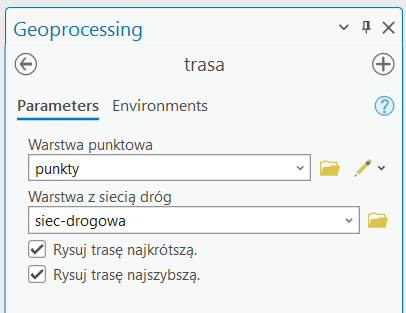
\includegraphics[width=0.5\textwidth]{img/narzedzie-interfejs-trasa.png}
    \caption{Interfejs narzędzia do wyznaczenia trasy}
\end{figure}

\section{Przykłady działania algorytmu wyznaczającego trasy}
Dla kilku przykładowych tras punktów początkowych i startowych przeprowadzono analizę działania algorytmu wyznaczającego trasy. Porównano wyniki z trasami proponowanymi przez Google Maps.

\subsection{Przykład 1: Dworzec Główny - Galeria Copernicus}
Długość najkrótszej trasy wyniosła w stworzonym narzędziu 5.832 km, a czas przejazdu najszybszą trasą wyniósł 5 minut. Najszybsza trasa proponowana przez Google Maps była wolniejsza o 5 minut. 
Przebieg tras wyznaczonych przez stworzone narzędzie oraz Google Maps przedstawiono na poniższych rysunkach.

\begin{figure}[H]
    \centering
    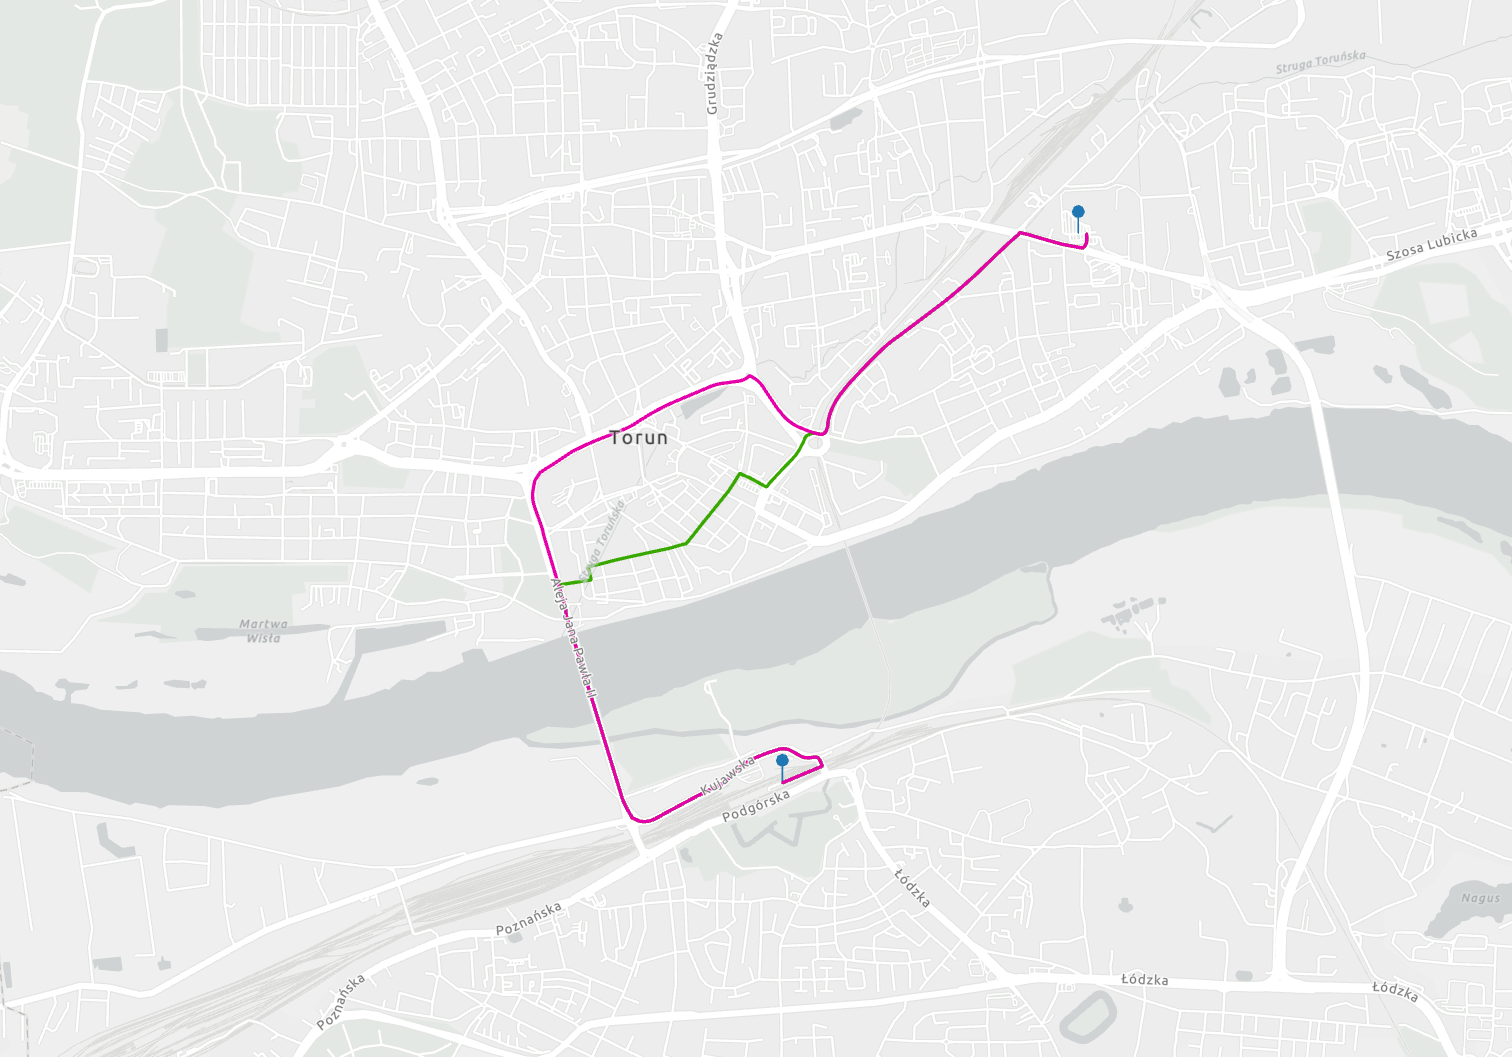
\includegraphics[width=1\textwidth]{img/glowny-copernicus.png}
    \caption{Trasy wyznaczone przez stworzone narzędzie (na zielono - trasa najkrótsza, na różowo - najszybsza)}
\end{figure}

\begin{figure}[H]
    \centering
    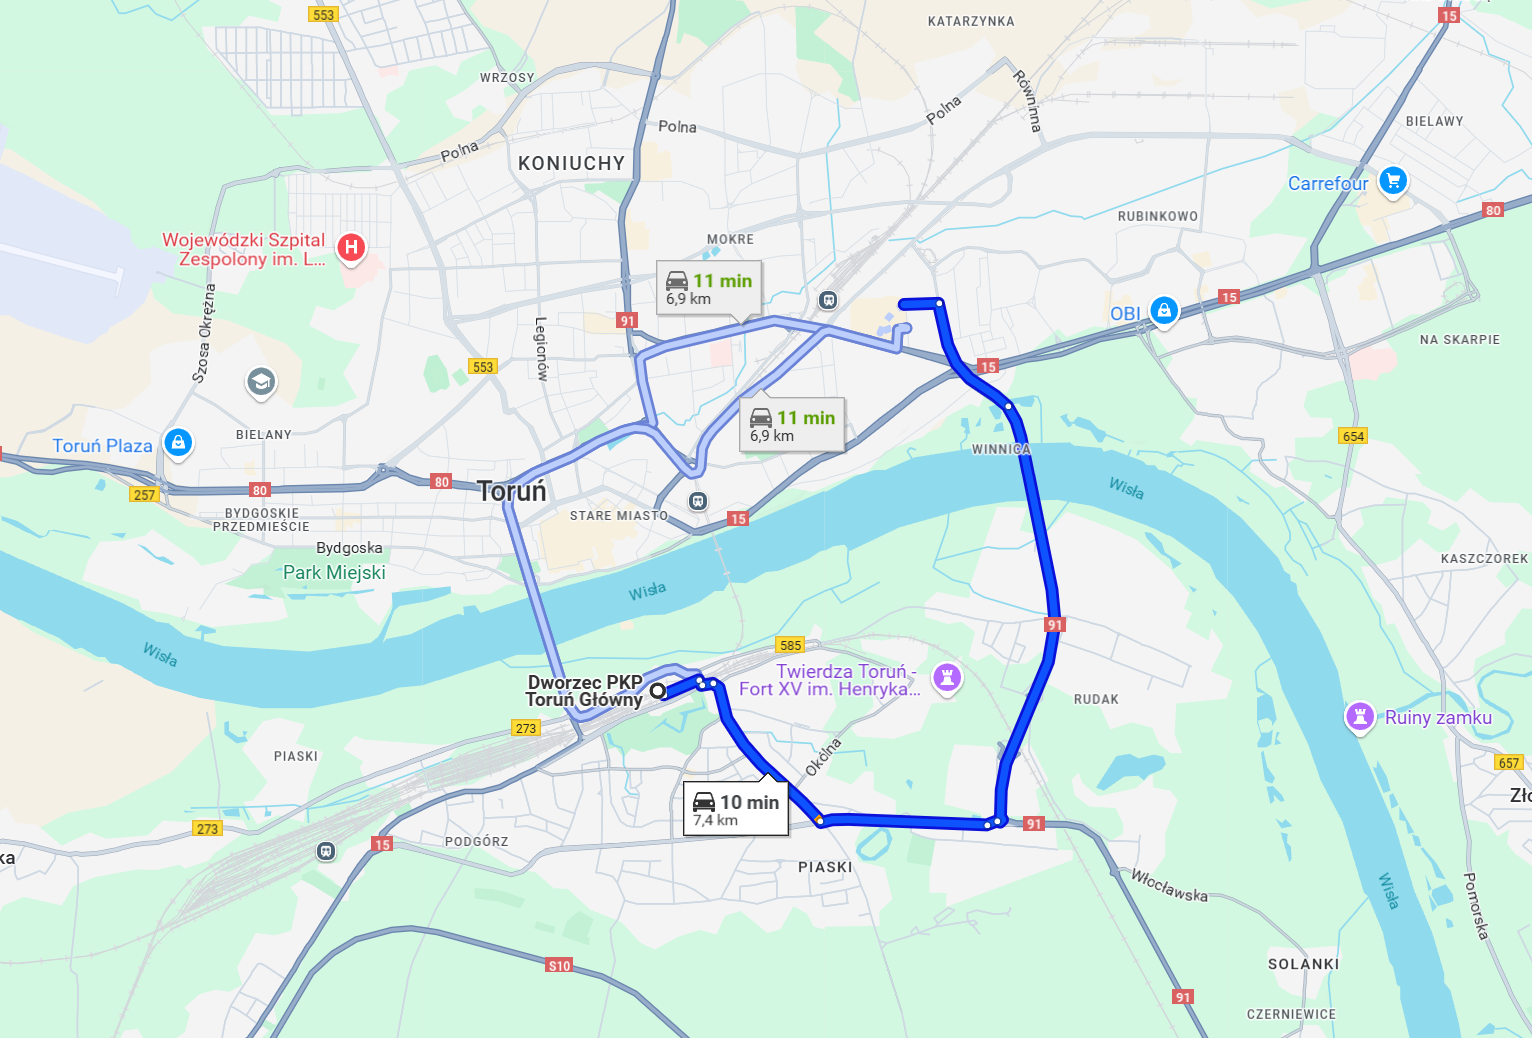
\includegraphics[width=1\textwidth]{img/glowny-copernicus-google.png}
    \caption{Trasy proponowane przez Google Maps}
\end{figure}

\subsection{Przykład 2: Motoarena - ROD Zielone Wzgórze}
Długość najkrótszej trasy wyniosła w stworzonym narzędziu 13.034 km, a czas przejazdu najszybszą trasą wyniósł 10 minut. Najszybsza trasa proponowana przez Google Maps różniła się od tej wyznaczonej przez stworzone narzędzie - najszybszy przejazd według Google Maps zająłby 20 minut.
Przebieg tras wyznaczonych przez stworzone narzędzie oraz Google Maps przedstawiono na poniższych rysunkach.

\begin{figure}[H]
    \centering
    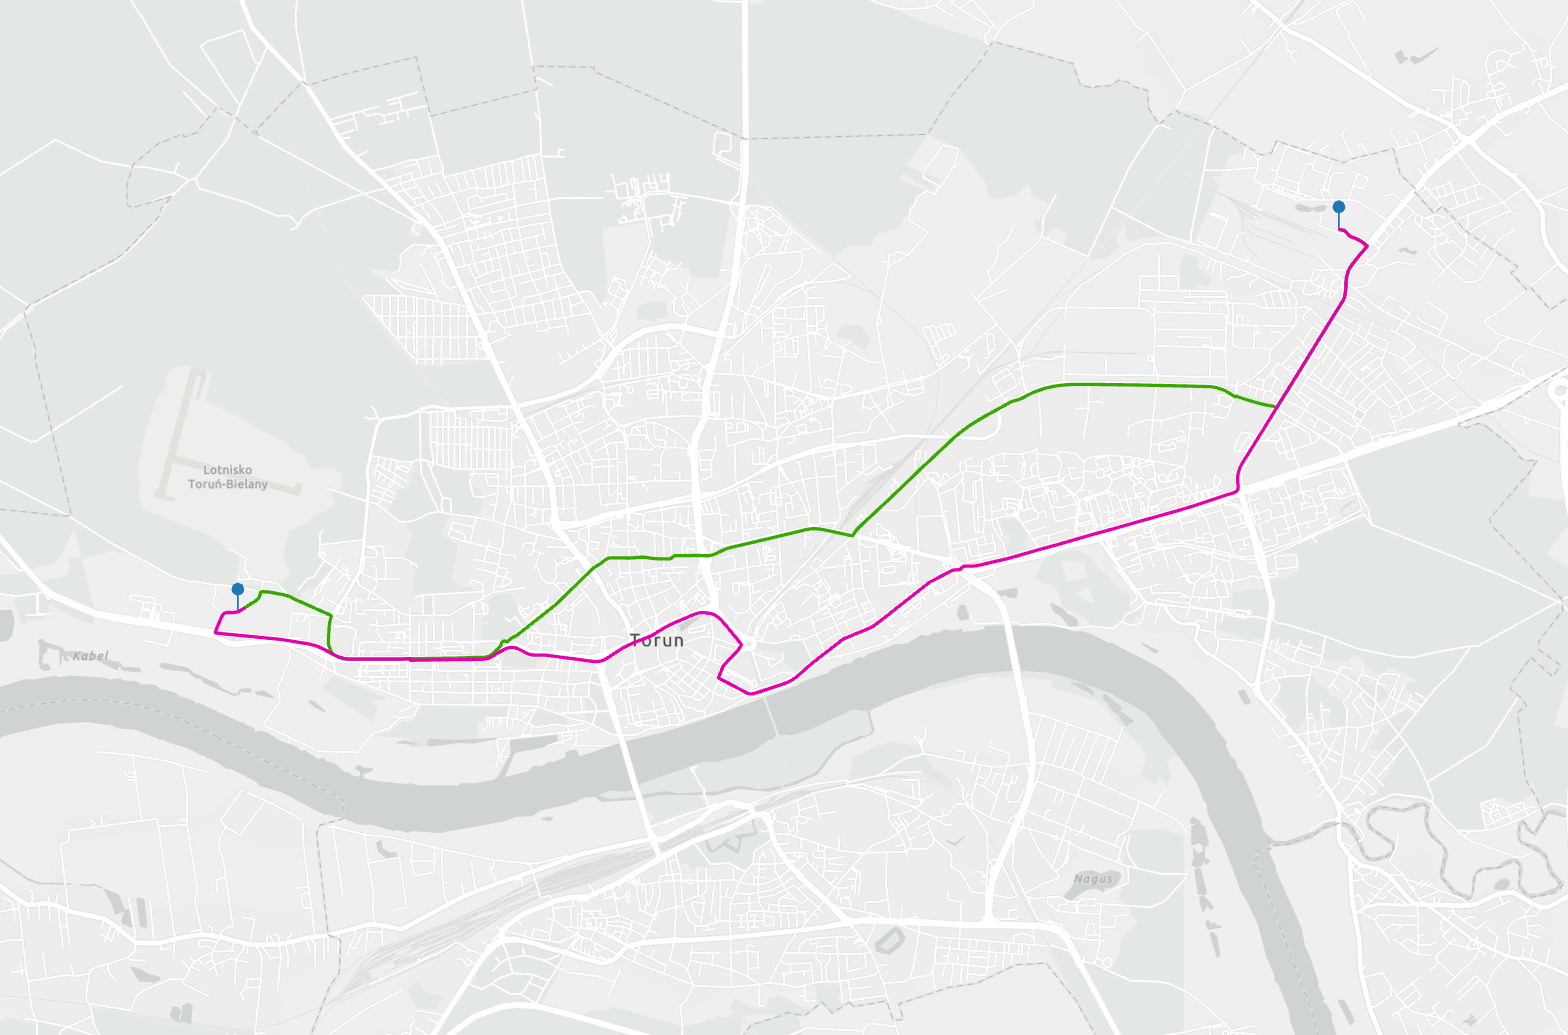
\includegraphics[width=1\textwidth]{img/motoarena-rod.png}
    \caption{Trasy wyznaczone przez stworzone narzędzie (na zielono - trasa najkrótsza, na różowo - najszybsza)}
\end{figure}

\begin{figure}[H]
    \centering
    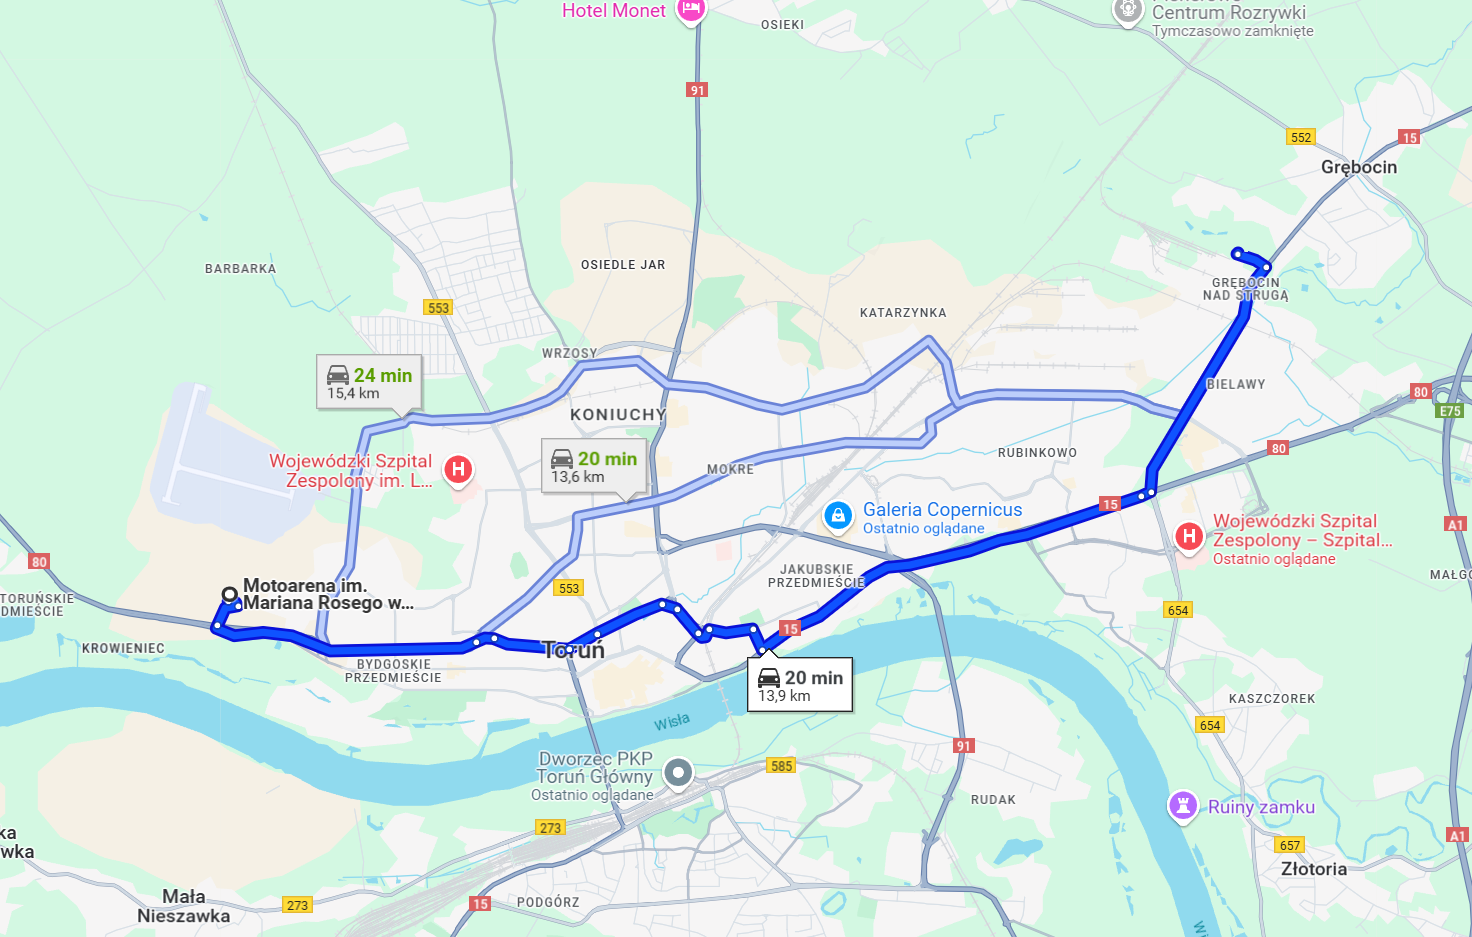
\includegraphics[width=1\textwidth]{img/motoarena-rod-google.png}
    \caption{Trasy proponowane przez Google Maps}
\end{figure}

\subsection{Przykład 3: Drogi z różną kierunkowością}
Kierunkowośc jest opisywana następująco:
\begin{itemize}
    \item 0 - droga przejezdna w obu kierunkach
    \item 1 - droga przejezdna tylko w kierunku zgodnym z geometrią
    \item 2 - droga przejezdna tylko w kierunku przeciwnym do geometrii
    \item 3 - droga nieprzejezdna
\end{itemize}

Do zaprezentowania działania algorytmu w zależności od kierunkowości przypisano wybranym ulicom różne wartości atrybuty kierunkowości. Informacje o kierunkowości danej
drogi przedstawiono na poniższym rysunku.
\begin{figure}[H]
    \centering
    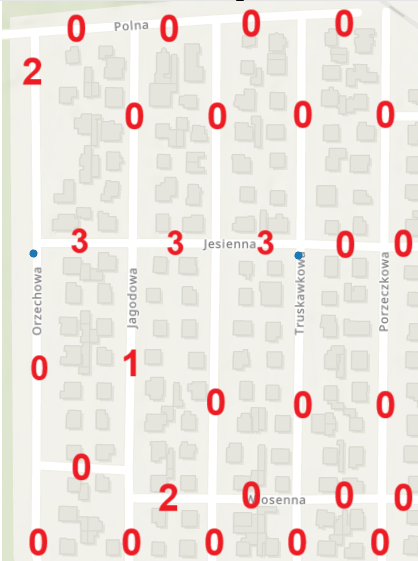
\includegraphics[width=0.45\textwidth]{img/kierunek-opis.png}
    \caption{Kierunkowość wybranych dróg}
\end{figure}

Różnicę w przebiegu trasy najkrótszej dla dwóch punktów zlokalizowanych przy ulicy Orzechowej i Truskawkowej przedstawiono poniżej.
\begin{figure}[H]
    \centering
    \begin{subfigure}[b]{0.45\textwidth}
        \centering
        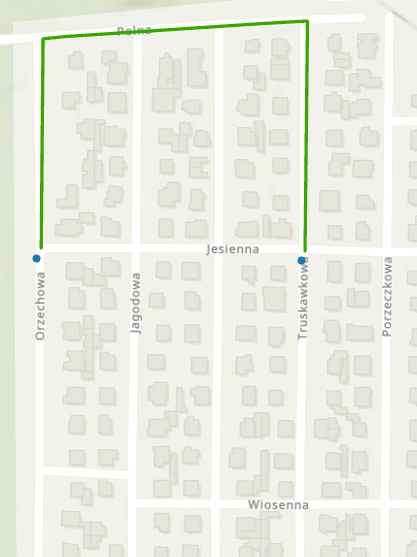
\includegraphics[width=\textwidth]{img/kierunek-orzechowa-truskawkowa.png}
        \caption{Trasa gdy punkt początkowy znajduje się przy ulicy Orzechowej}
    \end{subfigure}
    \hfill
    \begin{subfigure}[b]{0.45\textwidth}
        \centering
        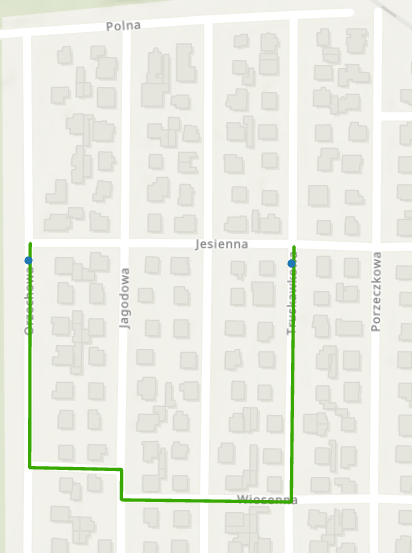
\includegraphics[width=\textwidth]{img/kierunek-truskawkowa-orzechowa.png}
        \caption{Trasa gdy punkt początkowy znajduje się przy ulicy Truskawkowej}
    \end{subfigure}
    \caption{Porównanie tras dla punktów przy ulicach Orzechowej i Truskawkowej}
\end{figure}

\subsection{Zmiany w prędkości}
Po przeanalizowaniu kilku przykładów zauważono, że różnice w czasie przejazdu między trasami wyznaczonymi przez stworzone narzędzie a trasami proponowanymi przez Google Maps są duże - stworzone narzędzie zwracało krótsze blisko o połowę czasy przejazdu. Aby uzyskać czas przejazdu bardziej podobny do rzeczywistego, zdecydowano się zmniejszyć prędkość ruchu dla każdej z kategorii dróg o połowę. Było to rozwiązanie, które bardziej uwzględniło istnienie czynników spowalniających ruch. Po zmianie prędkości, różnice w czasie przejazdu między trasami wyznaczonymi przez stworzone narzędzie a trasami proponowanymi przez Google Maps były mniejsze.

Dla przykładu 1, czas przejazdu najszybszą trasą zwiększył się z 5 do 10 minut, a dla przykładu 2 - z 10 do 19 minut.

\subsection{Czas działania}
Porównano czas wyznaczania danego rodzaju trasy i zauważono, że we wszystkich przypadkach czas wyznaczania trasy najszybszej jest dłuższy niż czas wyznaczania trasy najkrótszej.
Różnice nie były duże, ale zauważalne. W poniższych tabelach przedstawiono dokładne wartości liczbowe dla dwóch wybranych, wcześniej wizualizowanych przykładów.\\

\begin{table}[H]
\centering
\begin{tabular}{|c|c|}
\hline
Rodzaj trasy & Czas wyznaczania [s] \\
\hline
Najszybsza & 2,67 \\
\hline
Najkrótsza & 2,27 \\
\hline
\end{tabular}
\caption{Czas wyznaczania tras dla przykładu Dworzec Główny - Galeria Copernicus}
\end{table}

\begin{table}[H]
\centering
\begin{tabular}{|c|c|}
\hline
Rodzaj trasy & Czas wyznaczania [s] \\
\hline
Najszybsza & 2,93 \\
\hline
Najkrótsza & 2,61 \\
\hline
\end{tabular}
\caption{Czas wyznaczania tras dla przykładu Motoarena - ROD Zielone Wzgórze}
\end{table}

\section{Zasięg}
\subsection{Integracja z GIS}
Program do wyznaczania zasięgu również zintegrowano ze środowiskiem ArcGIS Pro. Użytkownik ma możliwość wybrania punktu początkowego na mapie, a następnie określenia czasu, w jakim chce dojechać do punktów z zasięgu. Program zwraca obszar, do którego można dojechać w wybranym czasie. Interfejs narzędzia został zaprezentowany na rysunku 8.

\begin{figure}[H]
    \centering
    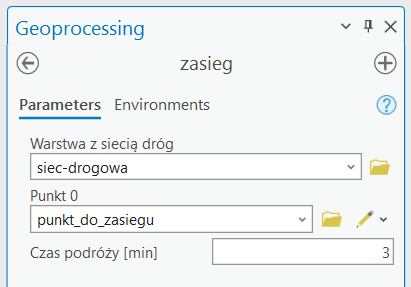
\includegraphics[width=0.5\textwidth]{img/narzedzie-interfejs-zasieg.png}
    \caption{ Interfejs narzędzia do wyznaczania zasięgu}
\end{figure}

\subsection{Przykłady działania}
Poniżej przedstawiono przykładowe zasięgi dla punktów początkowych zlokalizowanych na Rynku Staromiejskim i przy Bibliotece Uniwersyteckiej. Zasięgi zostały wyznaczone dla czasów 2 oraz 7 minut.
\begin{figure}[H]
    \centering
    \begin{subfigure}[b]{0.35\textwidth}
        \centering
        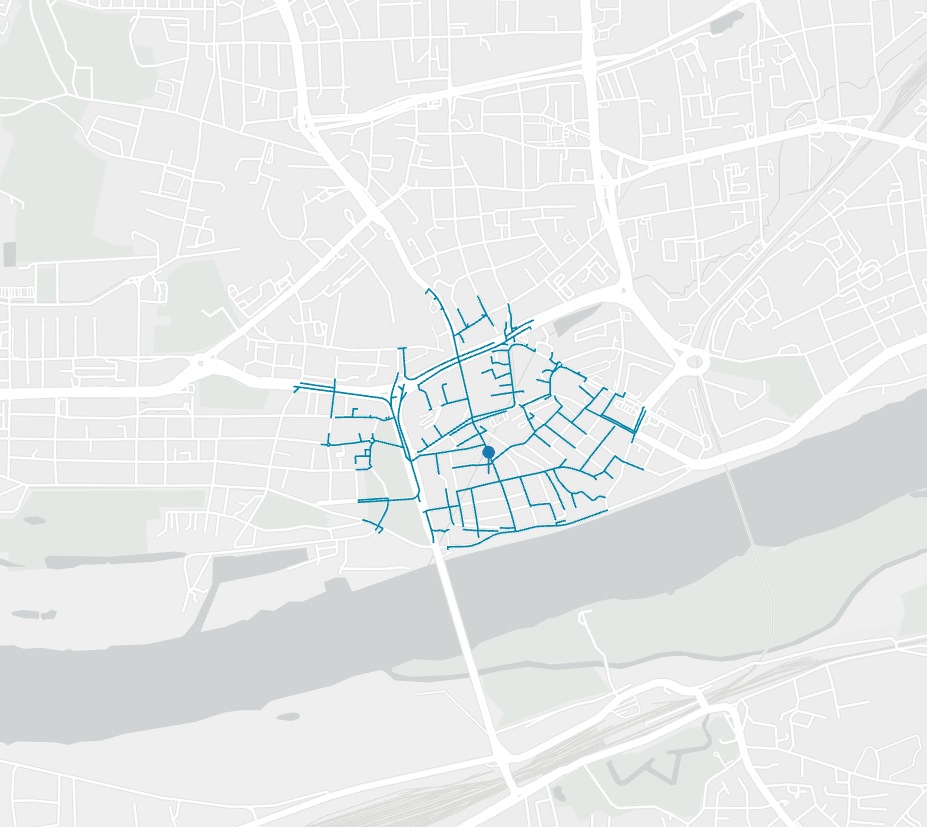
\includegraphics[width=\textwidth]{img/rynek-2-min.png}
        \caption{Trasy możliwe do pokonania w 2 minuty z punktu startowego na Rynku Staromiejskim}
    \end{subfigure}
    \hfill
    \begin{subfigure}[b]{0.55\textwidth}
        \centering
        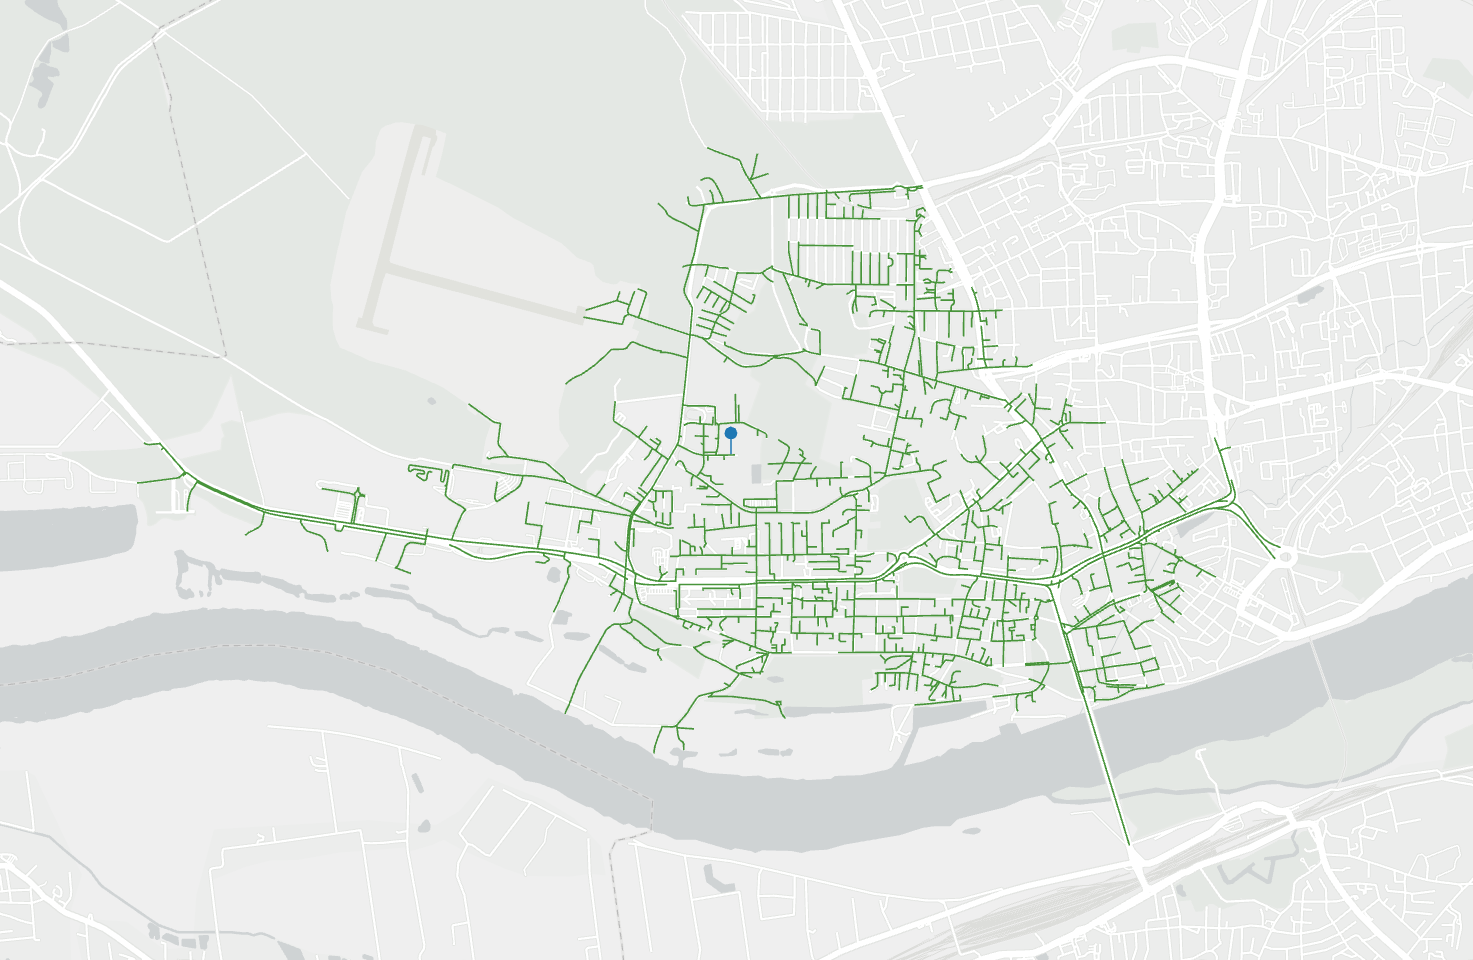
\includegraphics[width=\textwidth]{img/umk-7-min.png}
        \caption{Trasy możliwe do pokonania w 7 minut z punktu startowego przy Bibliotece Uniwesyteckiej}
    \end{subfigure}
    \caption{Przykładowe zasięgi}
\end{figure}

%\subsubsection{Przykład 3: Wydział Matematyki i Informatyki Uniwersytetu Mikołaja Kopernika}
Poniżej przedstawiono zasięg dla punktu początkowego zlokalizowanego przy Wydziale Matematyki i Informatyki Uniwersytetu Mikołaja Kopernika wyznaczony przez stworzone
narzędzie oraz przez Google Maps. Maksymalny czas dojazdu wynosił 15 minut.
\begin{figure}[H]
    \centering
    \begin{subfigure}[b]{0.45\textwidth}
        \centering
        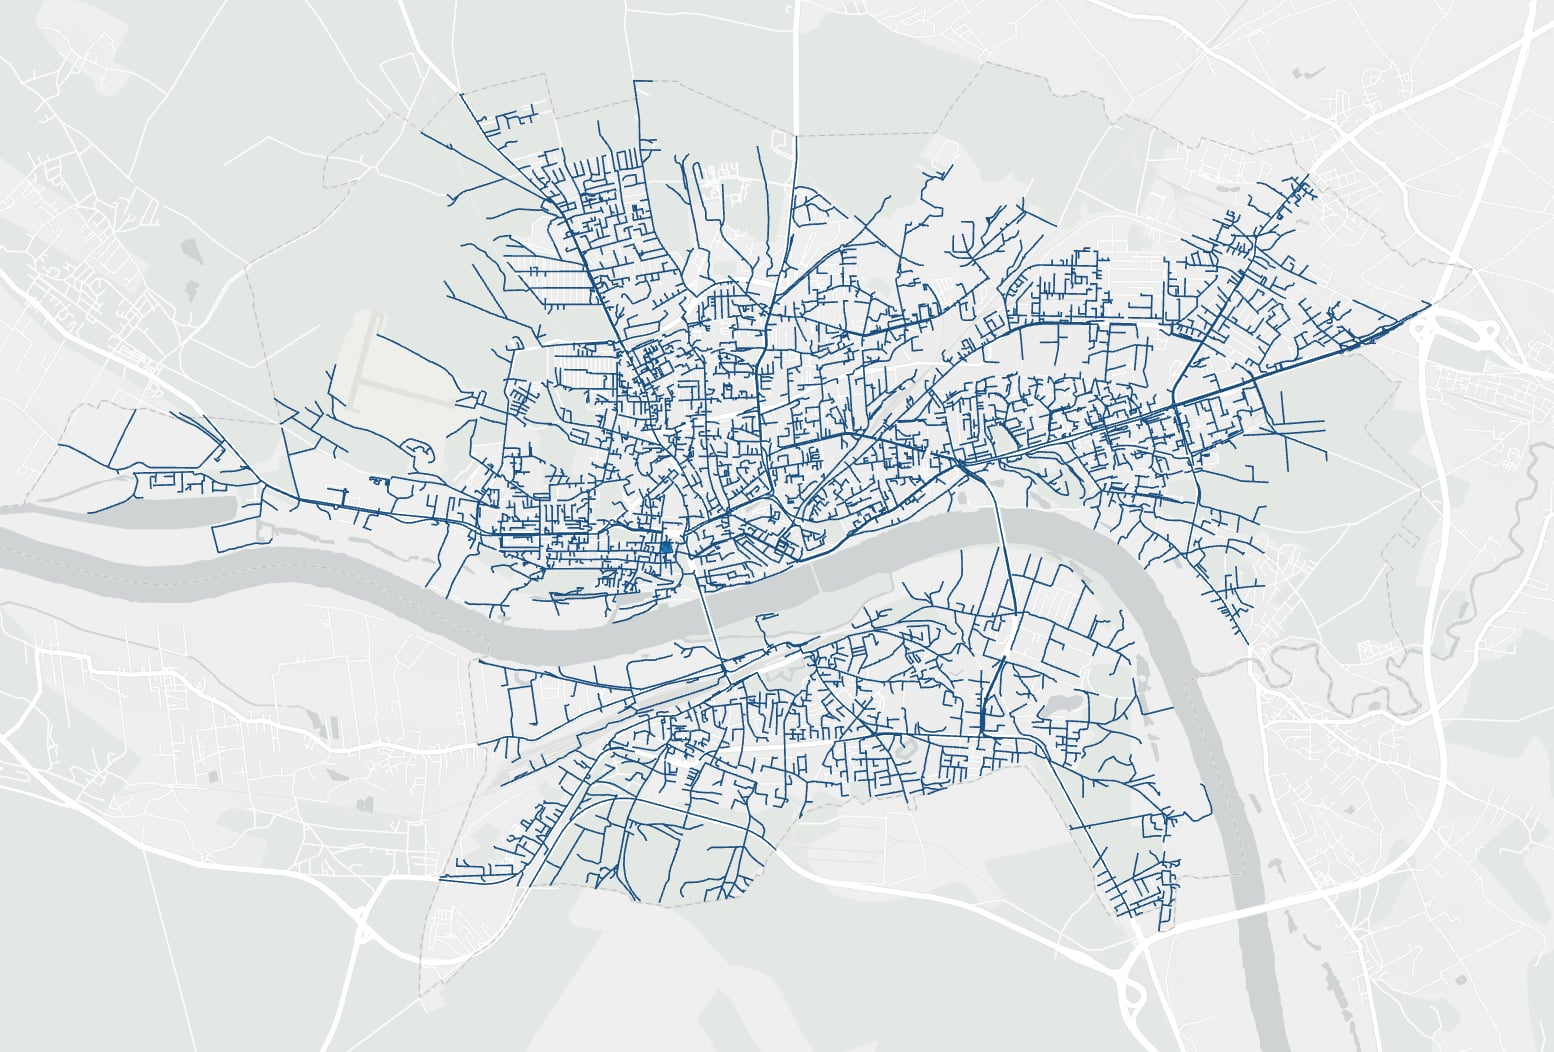
\includegraphics[width=\textwidth]{img/uniwersytet-15-min.png}
        \caption{Trasy możliwe do pokonania w 15 minut z punktu startowego przy Wydziale Matematyki i Informatyki Uniwersytetu Mikołaja Kopernika według stworzonego narzędzia}
    \end{subfigure}
    \hfill
    \begin{subfigure}[b]{0.45\textwidth}
        \centering
        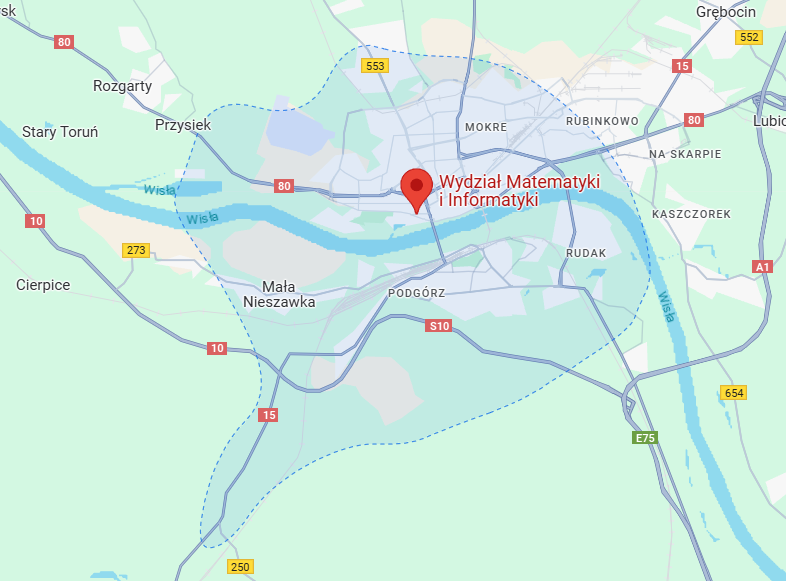
\includegraphics[width=\textwidth]{img/uniwersytet-15-min-google.png}
        \caption{Trasy możliwe do pokonania w 15 minut z punktu startowego przy Wydziale Matematyki i Informatyki Uniwersytetu Mikołaja Kopernika według Google Maps}
    \end{subfigure}
    \caption{Trasy możliwe do pokonania w 15 minut z punktu startowego przy Wydziale Matematyki i Informatyki Uniwersytetu Mikołaja Kopernika}
\end{figure}

\section{Wnioski}
Stworzony algorytm dobrze wyznacza trasę najkrótszą i najszybszą pomiędzy dwoma punktami. W przypadku zasięgu, algorytm zwraca większy obszar niż Google Maps.
Początkowe rozbieżności między wynikami uzyskanymi przez program a Google Maps wynikały z faktu, że zakładaliśmy poruszanie się z największą dopuszczalną prędkością, a w rzeczywistości poruszamy się wolniej.
Program nie uwzględnia ograniczeń w ruchu takich jak: zakazy ruchu, zakazy skrętu, rzeczywista kierunkowość dróg (kierunkowość dróg niepozwalająca na przejazd została przez 
nas nadana jedynie wybranym drogom). Nie mamy również informacji o aktualnym natężeniu ruchu, co znacząco wpływa na czas przejazdu.\\
Podczas pracy napotkano problemy związane z zbyt długim działaniem programu. Bardzo ważne jest stosowanie struktur danych, które zapewnią odpowiednią złożoność czasową. 
Podczas pracy ze zbiorami danych przestrzennych należy zwrócić uwagę na ich spójność. W naszym przypadku zdarzało się, że wierzchołki były oddalone od siebie o znikomą odległość, co powodowało, że algorytm działał niepoprawnie. W celu eliminacji tego problemu należało traktować takie wierzchołki jako jeden.\\
Opracowane rozwiązanie zostało stworzone w sposób, który umożliwia pracę z otrzymanymi danymi pochodzącymi z bazy BDOT. W przyszłości 
możnaby uczynić je bardziej uniwersalnym, umożliwiającym pracę z danymi z innych źródeł i/lub zawierającymi inne informacje (np. danymi z OSM,
które nie mają atrybutu \textit{klasaDrogi}). 
Używanie w funkcji heurystki największej możliwej prędkości poruszania się, powoduje, że algorytm analizuje więcej dróg. To sprawia że czas wyznaczenia trasy najszybszej jest dłuższy od czasu wyznaczenia trasy najkrótszej.

\section{Referencje}
[1] Amit Patel, Implementation of A*, redblobgames.com 2020 [dostęp: 8 grudnia 2024]. Dostępny w internecie: \url{https://www.redblobgames.com/pathfinding/a-star/implementation.html}
\end{document}
